\section{Tecnología \glsentryshort{iot}}
\label{iot}

La premisa básica de la tecnología \gls{iot} \cite{iotreview} conectar cualquier dispositivo que tenga cierta capacidad de cómputo. Esto significa que los objetos que actualmente no están conectados a Internet, estarán conectados de manera que puedan comunicarse e interactuar con personas y otros objetos. \\
\par

La tecnología \gls{iot} es una transición tecnológica en la que los dispositivos al ser dotados de inteligencia por estar conectados a Internet podrán proveer de entornos inteligentes a los humanos.  Cuando los objetos puedan ser controlados a distancia a través de una red, se habilitará una integración más estrecha entre el mundo físico y las máquinas, permitiendo mejoras en las áreas de medicina, automatización y logística \cite{7073822}.\\
\par

El ecosistema \gls{iot} es amplio, e incluso se puede parecer un poco caótico debido a la gran cantidad de componentes y protocolos que abarca. Es recomendable en vez de ver el \gls{iot} como un termino único, verlo como un paraguas de varios conceptos, protocolos y tecnologías, enfocados a un mismo propósito de interconectar ``Cosas" a Internet. Si bien la amplia mayoría de elementos \gls{iot} están diseñados para aportar numerosos beneficios en las áreas de productividad y automatización, al mismo tiempo introducen nuevos desafíos, como por ejemplo la gestión de la gran cantidad de dispositivos que van a aparecer en las redes, y la cantidad de datos y mensajes que todos estos generaran \cite{iotreview}.

\subsection{Arquitectura}

Aunque en el ecosistema hay diferentes \textit{stacks} de protocolos, todos ellos se pueden resumir en la siguiente arquitectura básica \cite{iotreview}.

\begin{itemize}
    \item \textit{Perception Layer}, en esta capa se da un significado físico a cada objeto. Consiste en sensores de diferentes tipos como etiquetas RFID, sensores IR u otras redes de sensores que podrían detectar la temperatura, la humedad, la velocidad y la ubicación, etc. Esta capa recolecta información útil a partir de los sensores vinculados a los objetos,  convierte dicha información en señales digitales que más tarde se delegarán a la Capa de Red para su posterior transmisión.
    
    \item \textit{Network Layer}, el propósito de esta capa es la de recibir la información en
    forma de señales digitales desde la capa de Percepción y transmitirla a los sistemas de procesamiento en la capa de \textit{Middleware}. Esto se llevará a cabo a través de las distintas tecnologías de acceso como WiFi, BLE, WiMaX, ieee802154 y con protocolos como IPv4, IPv6, MQTT.
    
    \item \textit{Middlware Layer}, en esta capa se procesa la información recibida de todos los sensores. En esta capa se puede incluir las tecnologías como Cloud computing, o sistemas gestores,  que aseguran un acceso directo a bases de datos donde se puede almacenar toda la información recolectada. Teniendo una gran cantidad de información centralizada, generalmente se aplican sistemas de inteligencia artificial para procesar la información, y tomar decisiones predictivas totalmente automatizadas. Estos sistemas suelen ser utilizados para analizar el tiempo, contaminación o tráfico en las ciudades. 
    
    \item \textit{Application Layer}, la finalidad de  esta  capa es la de realizar las aplicaciones \gls{iot} para el usuario final. Estas aplicaciones se valdrán de los datos procesados para ofrecer funcionalidades al usuario final, por ejemplo, una aplicación del tiempo.
    
    \item \textit{Business Layer}, esta capa aunque es un poco abstracta, se suele añadir para representar la gestión de múltiples las aplicaciones y servicios \gls{iot}. 
\end{itemize}

% Foto 
\begin{figure}[ht]
    \centering
    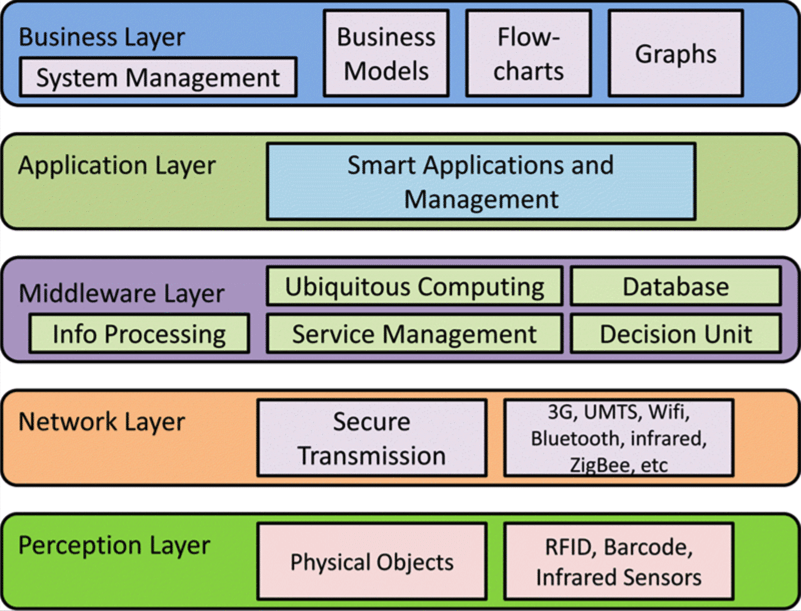
\includegraphics[width=6.5cm]{archivos/img/teoria/arch_edited.png}
    \caption{Arquitectura básica \glsentryshort{iot}}
    \label{fig:iotBasicArch}
\end{figure}

\subsection{Topologías}

Entre las tecnologías de acceso disponibles para conectar los dispositivos de \gls{iot}, dominan tres esquemas topológicos principales, estrella, malla y p2p. Para las tecnologías de acceso de largo y corto alcance, predomina la topología de estrella, como se puede encontrar en las redes datos móviles, LoRa y BLE. Las topologías en estrella utilizan una única estación base central para permitir las comunicaciones con los nodos finales. En cuanto a las tecnologías de mediano alcance, se pueden encontrar topologías en estrella, de p2p o en malla, como se ve en la figura \ref{fig:iotTopo}. Generalmente se suele hacer uso de un tipo de topología sobre otra en función de las limitaciones de los nodos que la conforman \cite{iotbook}.\\
\par

% Foto 
\begin{figure}[ht]
    \centering
    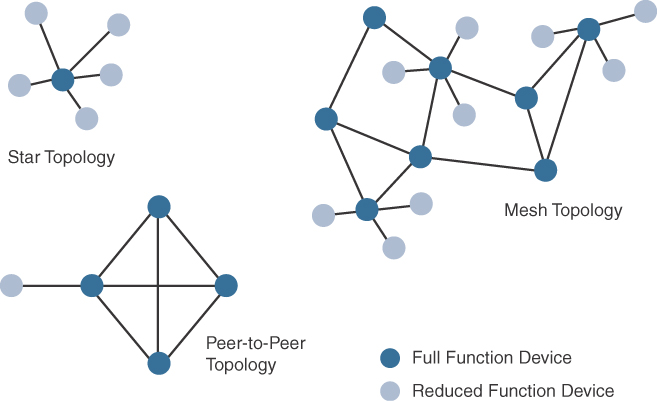
\includegraphics[width=7.5cm]{archivos/img/teoria/iot_topo.jpg}
    \caption{Tipos de topología con dispositivos \glsentryshort{iot} \cite{iotbook}}
    \label{fig:iotTopo}
\end{figure}


\subsection{Redes LLN}

Las redes de baja capacidad, conocidas como, \gls{lln}\footnote{\url{https://tools.ietf.org/html/rfc7228}}, se caracterizan por estar compuestas de dispositivos (sensores, motas) con limitaciones de memoria, batería y procesamiento. Dichos nodos, se interconectarán haciendo uso de distintos de tipos de enlace, como por ejemplo \texttt{ieee802154} ó LowPower-WiFi \cite{llnrfc}. Este tipo de redes pueden estar presentes en distintos campos de aplicación, entre las que se incluyen asistencia sanitaria, monitorización industrial, redes de sensores, etc.   \\

\par
Otra condición de las redes \gls{lln}, son las pérdidas en capa física debidas a las interferencias y variabilidad de los ``complicados" entornos radio donde estarán desplegadas dichas redes. Por ello, y teniendo en cuenta que los nodos que formarán parte de las redes \gls{lln} serán de baja capacidad, es necesario que los protocolos utilizados en esta red sean capaces de optimizar al máximo los recursos de los dispositivos \cite{iotbook}. 

\subsubsection{IEEE 802.15.4}

El estándar \texttt{ieee802154}\footnote{\url{https://tools.ietf.org/id/draft-ietf-lwig-terminology-05.html}} define la tecnología acceso a un entorno inalámbrico (\textit{phy} y \textit{mac}) para dispositivos de baja capacidad (limitados en batería y capacidad de transmisión). Este estándar se caracteriza por la optimización de los recursos del nodo en cuestión, consiguiendo una duración prolongada de la batería, además, esta tecnología de acceso permite un fácil uso utilizando un \textit{stack} de protocolos compacto, al tiempo que sigue siendo simple y flexible. Por todas estas características, el estándar \texttt{ieee802154} es usado en la mayoría de \textit{stack} de protocolos enfocados al \gls{iot}. Uno de los más utilizados es el \textit{stack} 6LoWPAN, definido por el \gls{ietf}, consiste en una capa de adaptación de IPv6 sobre las capas del estándar \texttt{ieee802154} (Ver figura \ref{fig:6lowapan}) \cite{6lowpan}.\\
\par

\vspace{0.5cm}

% Foto 
\begin{figure}[ht]
    \centering
    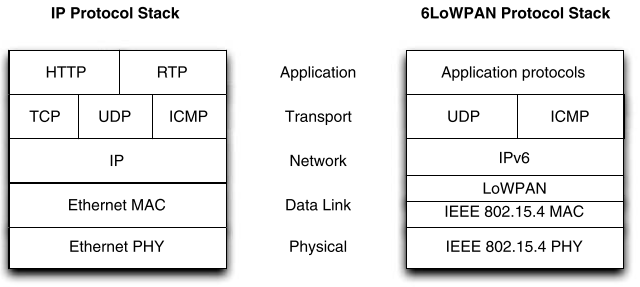
\includegraphics[width=12cm]{archivos/img/teoria/6LoWPAN-Protocol-Stack.png}
    \caption{Pila de protocolos 6LoWPAN \cite{6lowpan}}
    \label{fig:6lowapan}
\end{figure}

